%%%%%%%%%%%%%%%%%%%%%%%%%%%%%%%%%%%%%%%%%
% a0poster Portrait Poster
% LaTeX Template
% Version 1.0 (22/06/13)
%
% The a0poster class was created by:
% Gerlinde Kettl and Matthias Weiser (tex@kettl.de)
% 
% This template has been downloaded from:
% http://www.LaTeXTemplates.com
%
% License:
% CC BY-NC-SA 3.0 (http://creativecommons.org/licenses/by-nc-sa/3.0/)
%
%%%%%%%%%%%%%%%%%%%%%%%%%%%%%%%%%%%%%%%%%

%----------------------------------------------------------------------------------------
%	PACKAGES AND OTHER DOCUMENT CONFIGURATIONS
%----------------------------------------------------------------------------------------

\documentclass[a0,portrait]{a0poster}

\usepackage{multicol} % This is so we can have multiple columns of text side-by-side
\columnsep=100pt % This is the amount of white space between the columns in the poster
%\columnseprule=3pt % This is the thickness of the black line between the columns in the poster

\usepackage[svgnames]{xcolor} % Specify colors by their 'svgnames', for a full list of all colors available see here: http://www.latextemplates.com/svgnames-colors

\usepackage{times} % Use the times font
%\usepackage{palatino} % Uncomment to use the Palatino font

\usepackage{graphicx} % Required for including images
\graphicspath{{figs/}} % Location of the graphics files
\usepackage{booktabs} % Top and bottom rules for table
\usepackage[font=small,labelfont=bf]{caption} % Required for specifying captions to tables and figures
\usepackage{amsfonts, amsmath, amsthm, amssymb} % For math fonts, symbols and environments
\usepackage{wrapfig} % Allows wrapping text around tables and figures
\usepackage{subcaption}
\usepackage{bm}
\usepackage{amsmath,amssymb}
\usepackage{listings}

\newcommand{\gpmem}{\texttt{gpmem}}
\newcommand{\emu}{{\textrm{emu}}}
\newcommand{\restr}{{\textrm{restr}}}
\newcommand{\true}{{\textrm{true}}}
\newcommand{\rmnew}{{\textrm{new}}}
\newcommand{\past}{{\textrm{past}}}
\newcommand{\prior}{{\textrm{prior}}}
\newcommand{\noisy}{{\textrm{noisy}}}
\newcommand{\noise}{{\textrm{noise}}}

\newcommand{\Acal}{\mathcal{A}}
\newcommand{\R}{\mathbb{R}}

\newcommand{\abf}{\mathbf{a}}
\newcommand{\fbf}{\mathbf{f}}
\newcommand{\rbf}{\mathbf{r}}
\newcommand{\wbf}{\mathbf{w}}
\newcommand{\xbf}{\mathbf{x}}
\newcommand{\ybf}{\mathbf{y}}
\newcommand{\Kbf}{\mathbf{K}}
\newcommand{\Ibf}{\mathbf{I}}

\newcommand{\pn}[1]{\left( #1 \right)}
\newcommand{\bkt}[1]{\left[ #1 \right]}
\newcommand{\br}[1]{\left\{ #1 \right\}}
\newcommand{\abs}[1]{\left\lvert #1 \right\rvert}
\newcommand{\Ebkt}[2][]{\mathbb{E}_{#1}\bkt{#2}}
\newcommand{\mvert}{\ \middle\vert\ }

\DeclareMathOperator*{\Cov}{Cov}
\begin{document}

%----------------------------------------------------------------------------------------
%	POSTER HEADER 
%----------------------------------------------------------------------------------------

% The header is divided into two boxes:
% The first is 75% wide and houses the title, subtitle, names, university/organization and contact information
% The second is 25% wide and houses a logo for your university/organization or a photo of you
% The widths of these boxes can be easily edited to accommodate your content as you see fit
\begin{flushright}
\begin{minipage}[b]{0.25\linewidth}

\includegraphics[width=7cm]{mitlogo.png}
\hspace{1cm}

\includegraphics[width=8cm]{royalhollowaylogo.jpg}
\end{minipage} 
\end{flushright}

\vspace{2cm}

\begin{center}
\addtolength{\tabcolsep}{20pt} 
\veryHuge \textbf{Probabilistic Programming with Gaussian Process Memoization} \color{Black}\\[1.5cm] % Title
 \Large   \begin{tabular}{  c  c  c c}
           \textbf{Ulrich Schaechtle}  & \textbf{Ben Zinberg} & \textbf{Vikash K. Mansinghka} & \textbf{Kostas Stathis}\\ 
           Department of Computer Science & Computer Science \& AI Lab & Computer Science \& AI Lab & Department of Computer Science \\
           Royal Holloway, Univ. of London & Massachusetts Institute of Technology & Massachusetts Institute of Technology & Royal Holloway, Univ. of London \\
        \end{tabular}

\addtolength{\tabcolsep}{-2pt} 
\end{center}



\vspace{3cm} % A bit of extra whitespace between the header and poster content

%----------------------------------------------------------------------------------------

\begin{multicols}{2} % This is how many columns your poster will be broken into, a portrait poster is generally split into 2 columns

%----------------------------------------------------------------------------------------
%	ABSTRACT
%----------------------------------------------------------------------------------------

%\color{Navy} % Navy color for the abstract

\begin{abstract}
{\em Gaussian process memoizer} is a probabilistic programming technique that uses Gaussian processes to provides a statistical alternative to memorization. Memoizing a target procedure results in a “self-caching” wrapper that remembers previously computed values. Gaussian process memoization additionally produces a statistical emulator based on a Gaussian process whose predictions automatically improve whenever a new value of the target procedure becomes available. The work also introduces  an efficient implementation, named {\tt gpmem}, that can use kernels given by a broad class of probabilistic programs. The flexibility of {\tt gpmem} is illustrated via three applications: (i) GP regression with hierarchical hyper-parameter learning, (ii) Bayesian structure learning and (iii) a bandit formulation of Bayesian optimization.
\end{abstract}


\color{DarkSlateGray} % DarkSlateGray color for the rest of the content
%\color{SaddleBrown} % SaddleBrown color for the introduction
%----------------------------------------------------------------------------------------
%	GP Memoization
%----------------------------------------------------------------------------------------
\section*{GP Memoization: {\tt gpmem}}
\subsection*{Gaussian Processes}
For any finite set of inputs $\xbf$, the marginal prior on $f(\xbf)$ is the multivariate Gaussian $f(\xbf) \sim \mathcal{GP}(0, k(\xbf,\xbf))$,
where $k(\xbf,\xbf') = \Cov_f\pn{f(\xbf), f(\xbf')}$ is the covariance function, a.k.a.\ kernel.
The marginal likelihood can be expressed as:
\begin{equation*}
\label{eq:marg}
p\pn{f(\xbf) = \ybf \mvert \xbf} = \int p\pn{f(\xbf) = \ybf \mvert f, \xbf}\, p(f|\xbf) \, df
\end{equation*}
where here $p(f|\xbf) = p(f) \sim \mathcal{GP}(m,k)$ since we assume no dependence of $f$ on $\xbf$.
We can sample a vector of unseen data $\ybf^* = f(\xbf^*)$ from the predictive posterior with
\begin{equation*}
\label{eq:gpsampler}
\ybf^* \sim \mathcal{N}(\bm{\mu},\bm{\Sigma}),
\end{equation*}
with $\bm{\mu} = k(\xbf,\xbf^*)\, k(\xbf^*,\xbf^*)^{-1}\, \ybf$ and $\bm{\Sigma} =  k(\xbf,\xbf) - k(\xbf,\xbf^*)k(\xbf^*,\xbf^*)^{-1} k(\xbf^*,\xbf)$'

\subsection*{Memoization}
Memoization is the practice of storing previously computed values of a function so that future calls
with the same inputs can be evaluated by lookup rather than re-computation. Gaussian Process memoization: 

\begin{itemize}
\setlength{\itemindent}{1cm}
 \item is a statistical alternative to standard memoization;
 \item changes semantics of a probabilistic program; and
 \item produces a statistical emulator whose predictions improve with memoization.
\end{itemize}


---------------------------------------------------------------------


%----------------------------------------------------------------------------------------
%	Bayesian GP
%----------------------------------------------------------------------------------------
\section*{Bayesian GP}

We show how we can use  {\tt gpmem} to reproduce Neal's Hierarchical Bayesian GP~\cite{neal1997monte} for data with outliers.
\begin{minipage}{\linewidth}
\footnotesize
\belowcaptionskip=-10pt
\begin{lstlisting}[frame=single,caption=Hierarchical  GP Smoothing,mathescape,label=alg:gphierarch,escapechar=']
[ASSUME alpha (mem (lambda (i)  (gamma  1 3 )))] $\in$ {hyper-parameters-$\Gamma$} 
[ASSUME beta  (mem (lambda (i)  (gamma  1 3 )))] $\in$ {hyper-parameters-$\Gamma$} 
[ASSUME l  (gamma (alpha 1) (beta 1))]   $\in$ {hyper-parameters} 
[ASSUME sf (gamma (alpha 2) (beta 2))]   $\in$ {hyper-parameters}
[ASSUME sigma (uniform 0 5 )]            $\in$ {hyper-parameters} % Fig. '\ref{fig:inference}'
% above: structured prior, Fig. '\ref{fig:NealpriorStruct}'
$\smash{k_{SE}(x,x^\prime) := \theta^2 \exp(-\frac{(x-x^\prime)^2}{2\ell^2})}$
$\smash{k_{WN}(x,x^\prime) := \sigma^2 \delta_{x,x^\prime}}$
[ASSUME k$_{SE}$ VentureFunction($k_{SE},\theta,\ell$) ]
[ASSUME k$_{WN}$ VentureFunction($k_{WN},\sigma$) ]
[ASSUME SE make-se (apply-function k$_{SE}$ l sf) ]
[ASSUME WN make-se (apply-function k$_{WN}$ sigma) ]
[ASSUME (list f_compute f_emu) (gpmem f_restr (function-plus SE WN) )]
[SAMPLE (f_emu (array 1 2 3))]  % prior, Fig. '\ref{fig:NealBO}'
for i=1 to n:
  [PREDICT (f_compute x[i])] % observing with a look-up function
[SAMPLE (f_emu (array 1 2 3))]  % after observation, Fig. '\ref{fig:NealAO}'
[INFER (REPEAT 100 
	(DO (MH {hyper-parameters} one 2)
	    (MH {hyper-parameters-$\Gamma$} one 2) ))]
[SAMPLE (f_emu (array 1 2 3))]  % posterior , Fig. '\ref{fig:NealAI}'
\end{lstlisting}
\end{minipage}

Observed data is generated with the following model: 
\begin{equation*}
f(x) =  0.3 + 0.4 x + 0.5 \sin(2.7x) + \frac{1.1}{(1+ x^2)} + \eta \;\;\; with\;\;\eta \sim \mathcal{N}(0,\sigma)
\end{equation*} where $\sigma$ is $0.1$ with probability $0.95$, $1$ otherwise.
\begin{center}
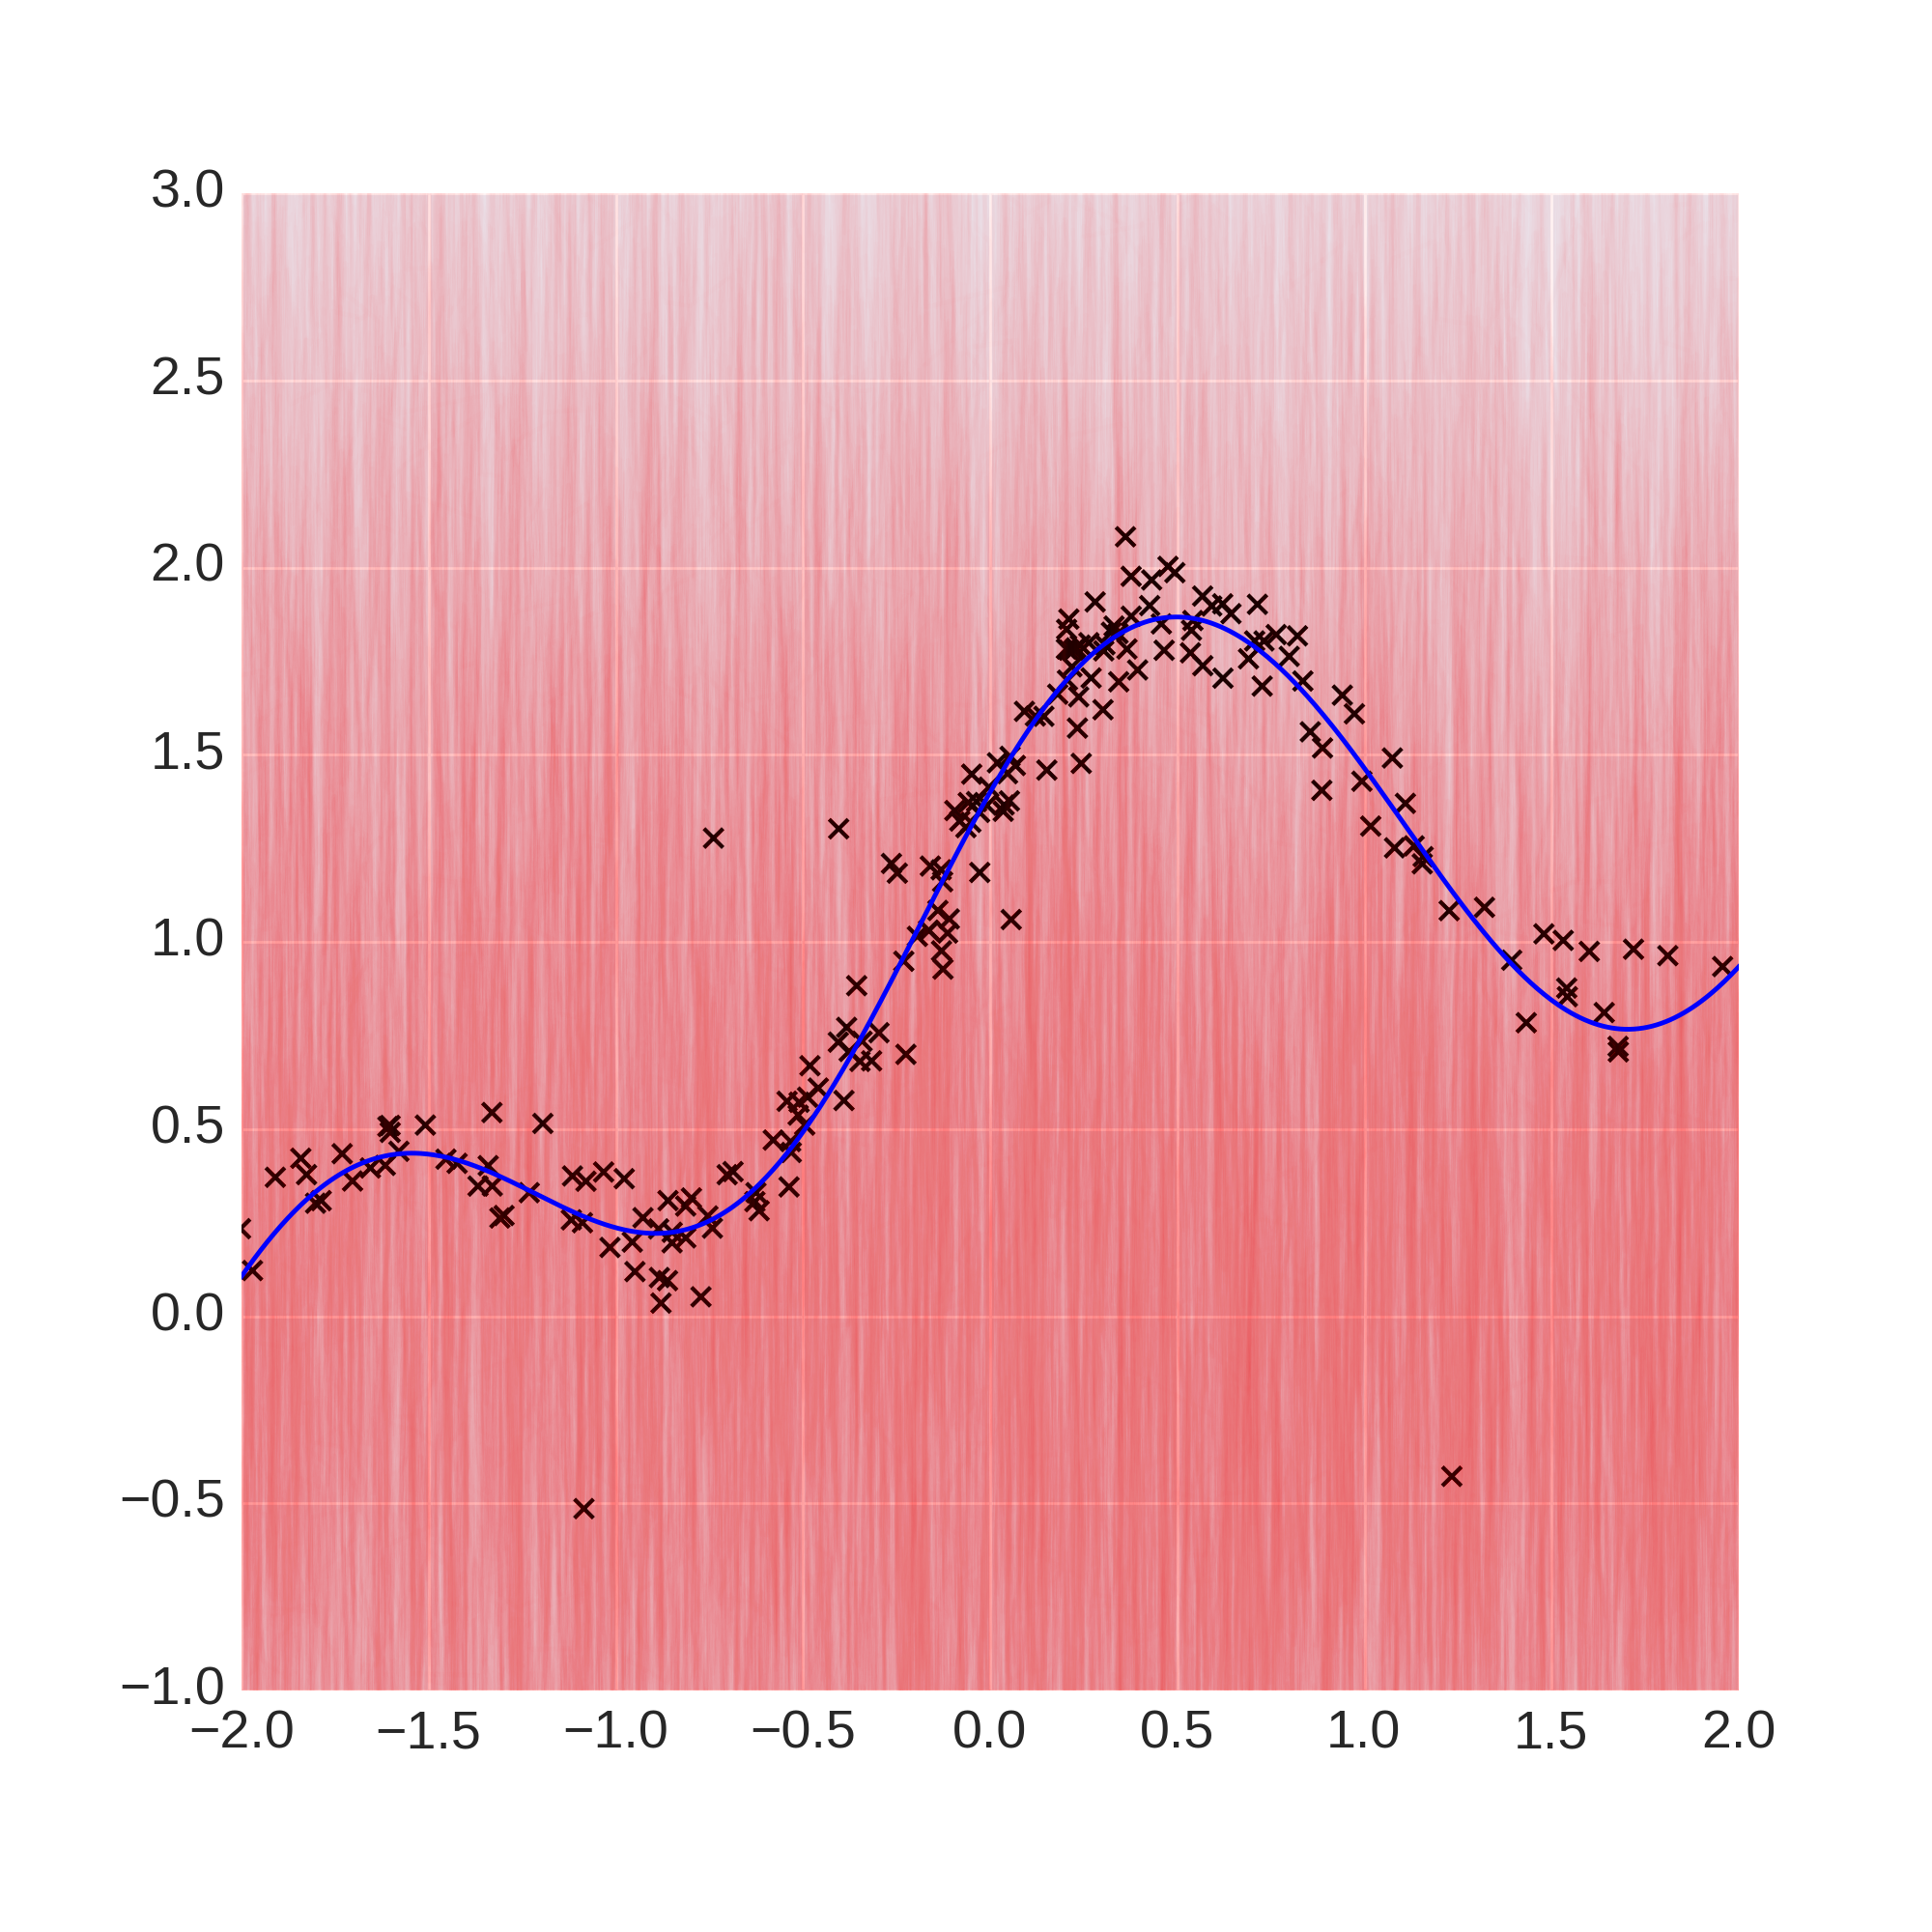
\includegraphics[width=7cm]{neal_se_1final.png}
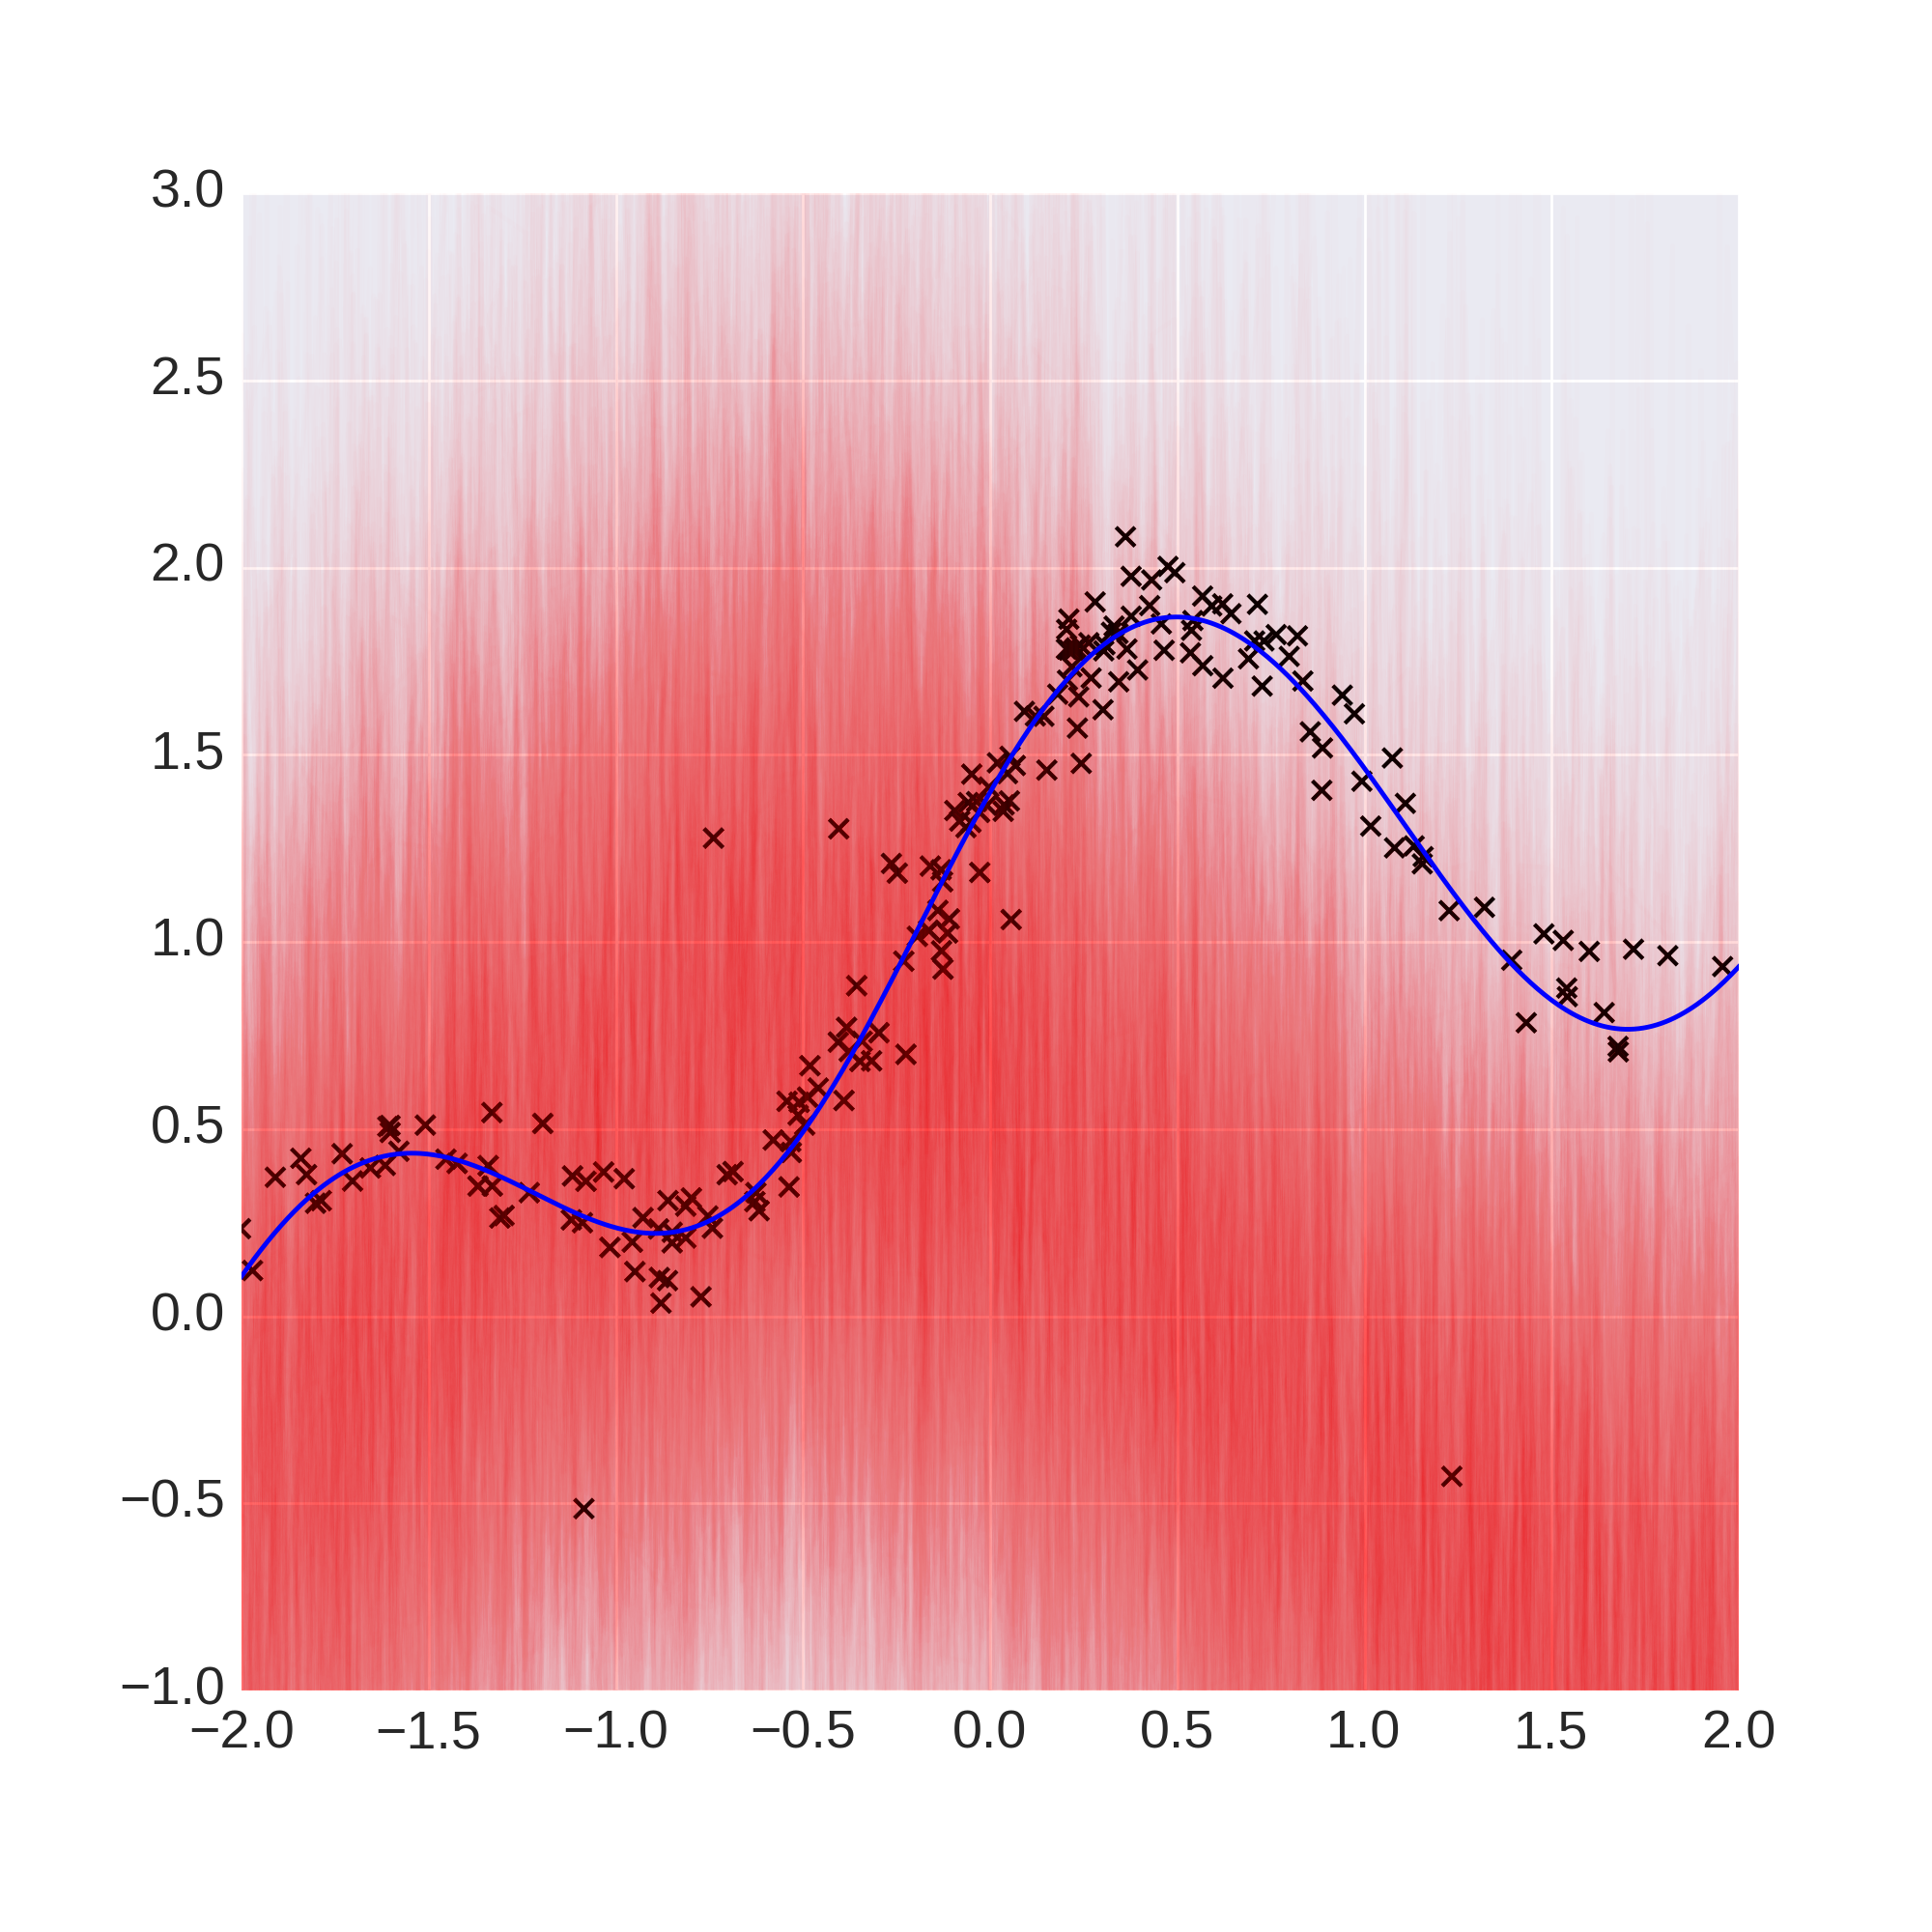
\includegraphics[width=7cm]{neal_se_2final.png}
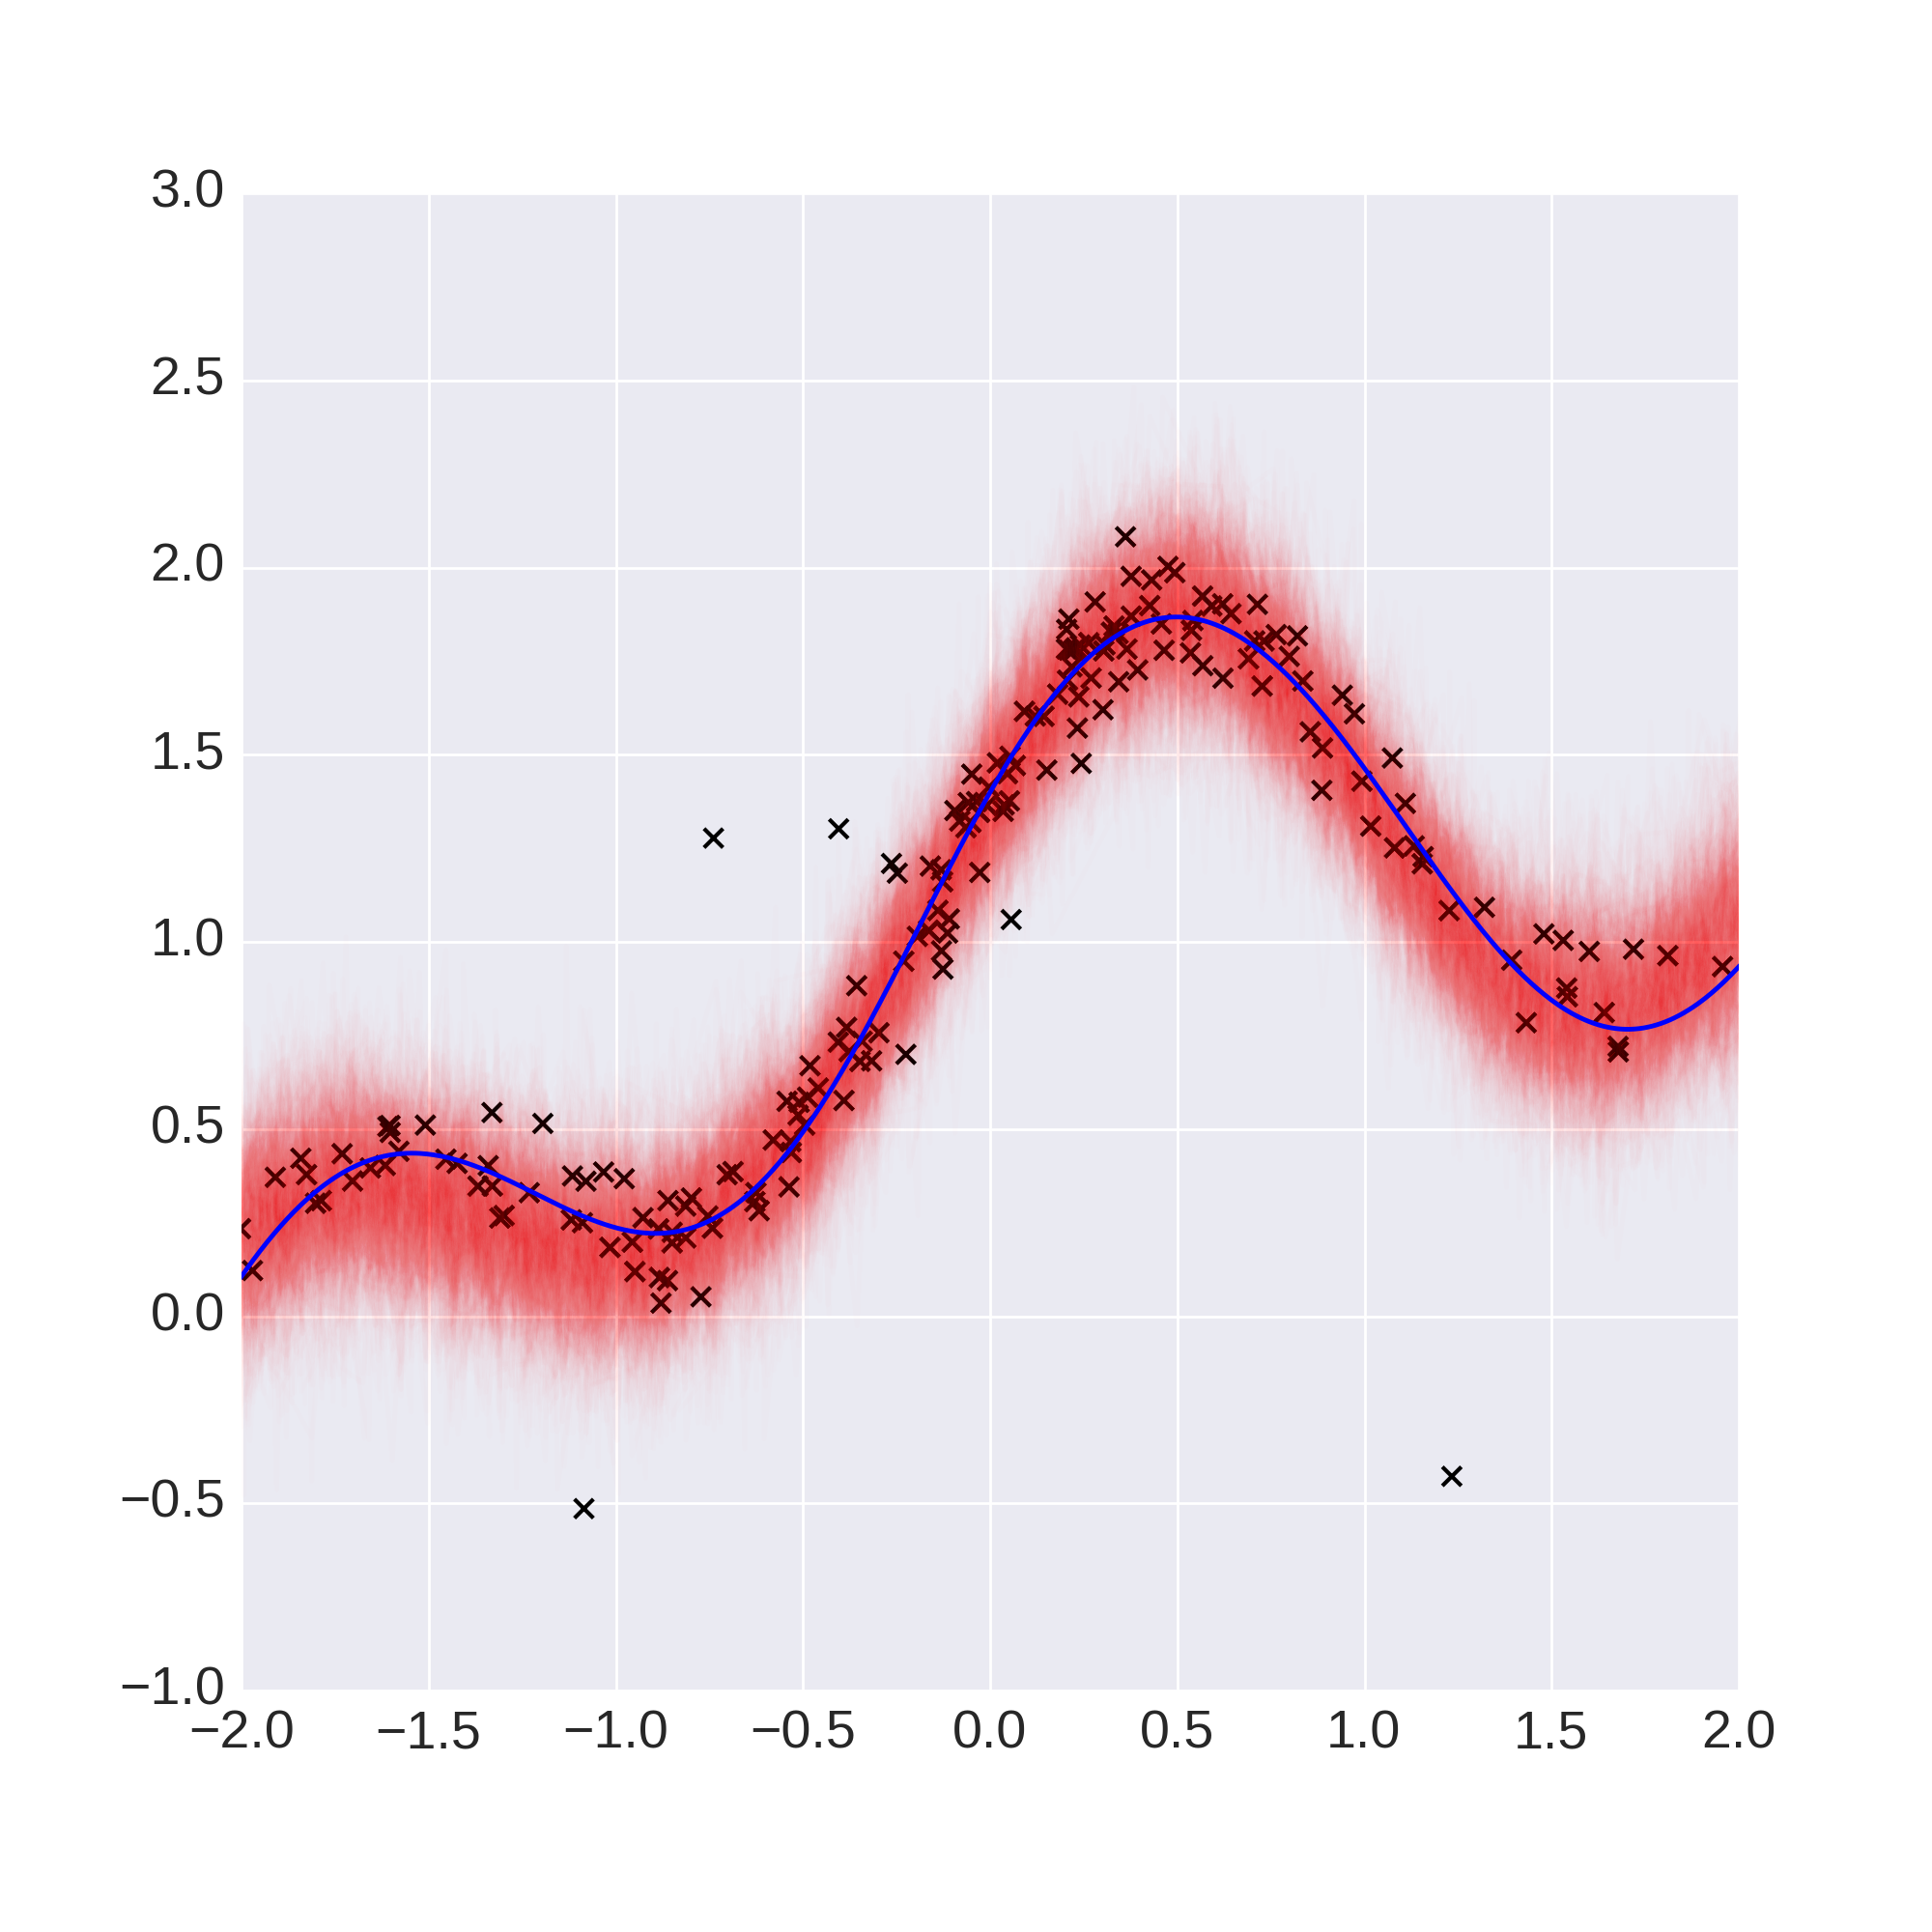
\includegraphics[width=7cm]{neal_se_3final.png}
\end{center}


% Left or right alignment is specified in the first bracket, the width of the table is in the second


%\begin{wraptable}{r}{15cm} 
\begin{wraptable}{r}{10cm} % Left or right alignment is specified in the first bracket, the width of the table is in the second
\begin{center}
%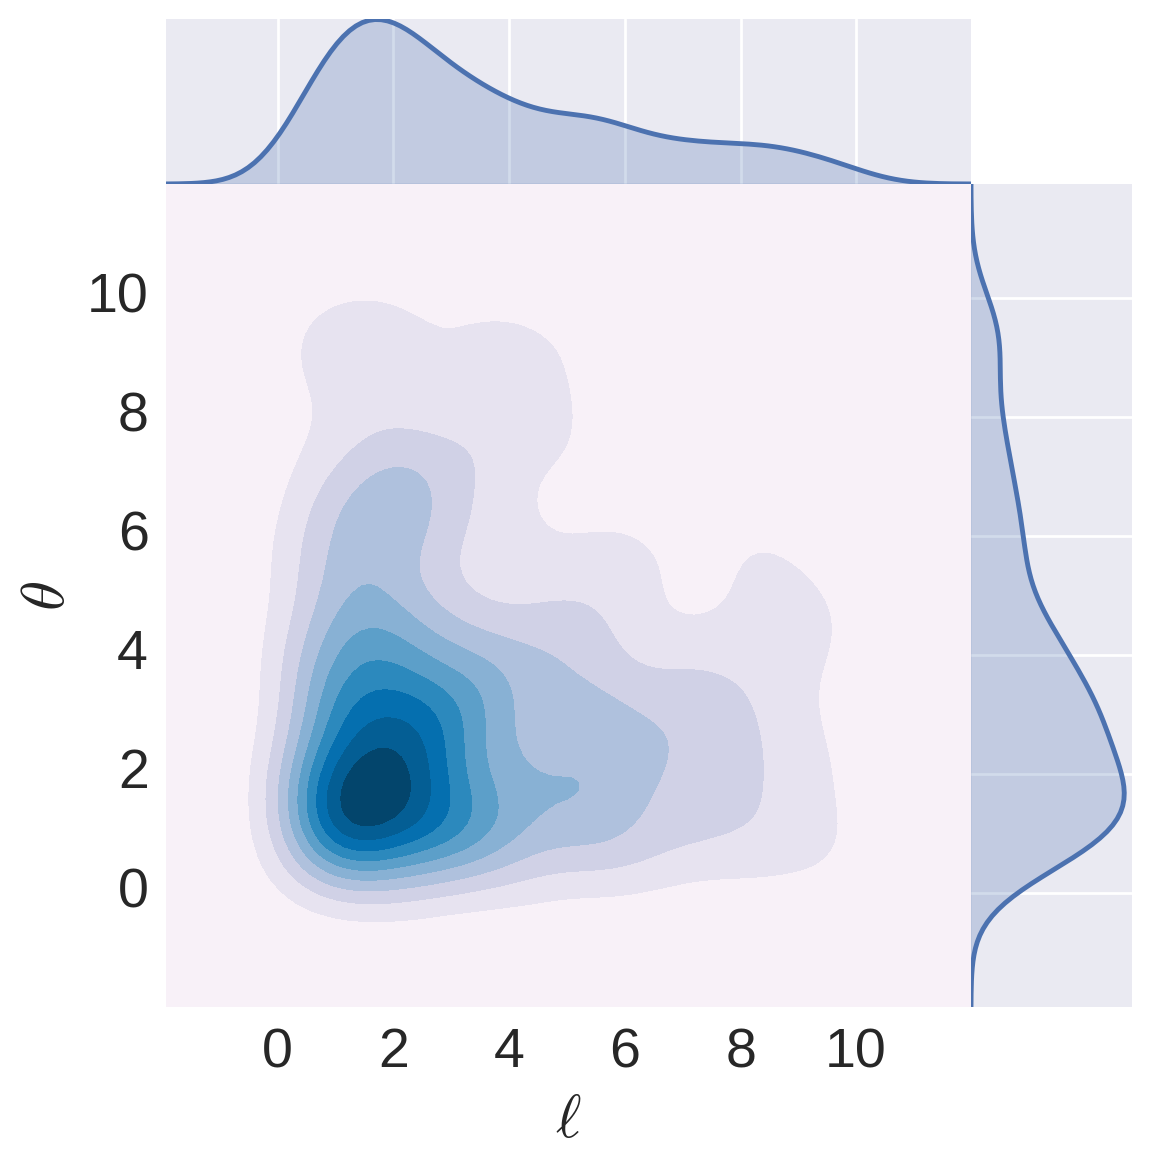
\includegraphics[width=10cm]{neal_contour_l_vs_sf_s__marginal_before.png}
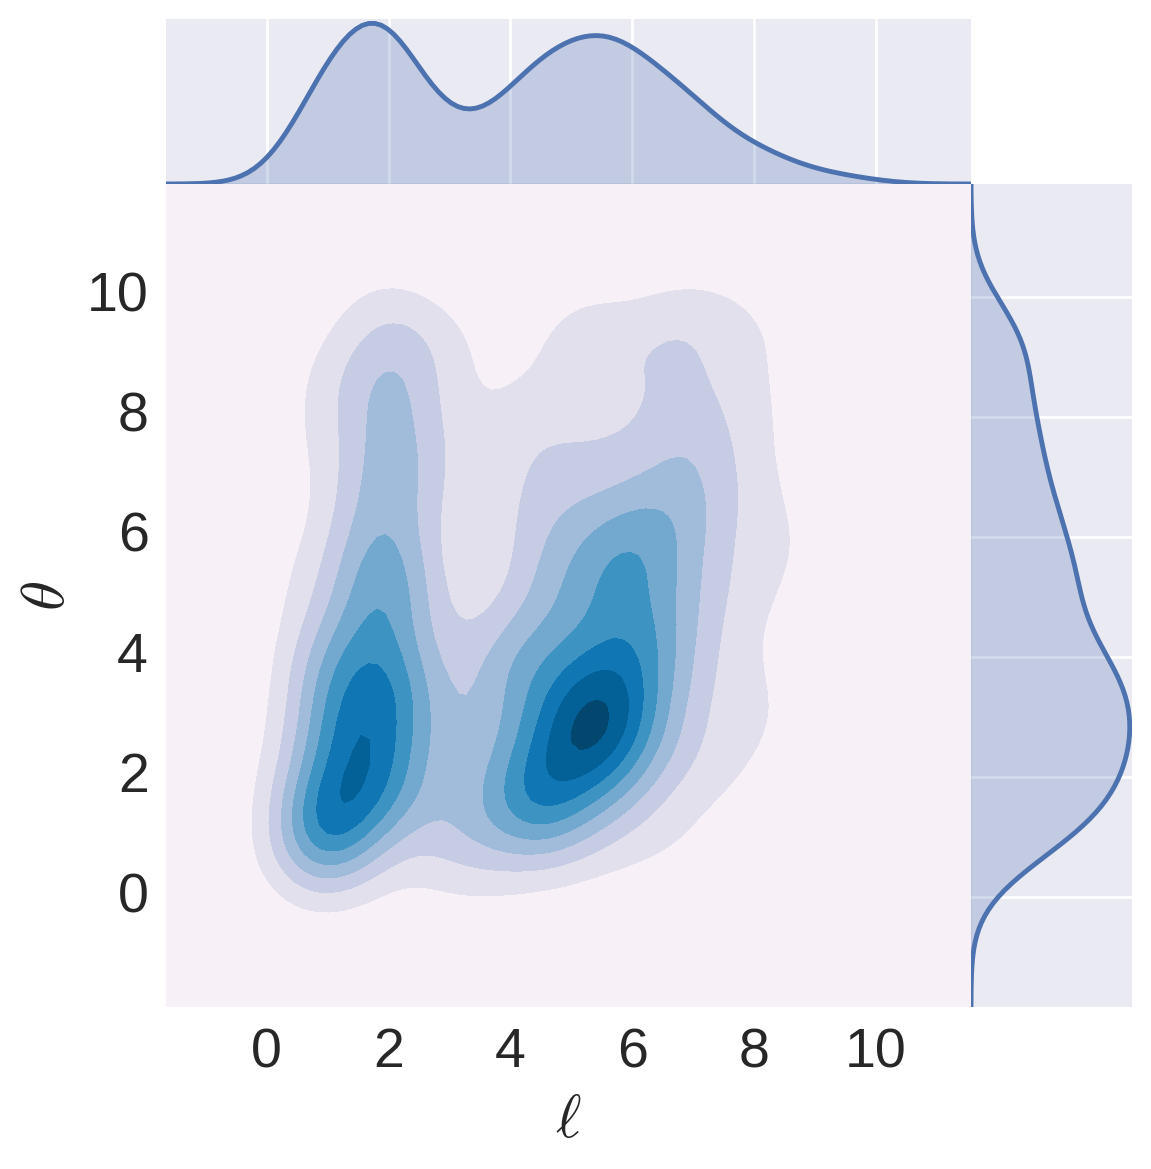
\includegraphics[width=10cm]{neal_contour_l_vs_sf_s__marginal_after.png} 
\end{center}
\end{wraptable}
 Above, we (left to right) we see predictions before data has been observed, after data has been observed, after we inferred over these observations. On the right, we see a contour plot and marginals of the the $\ell$ and $\theta$ hyper-parameters of the above program after inference (right).

-------------------------------------------------


%----------------------------------------------------------------------------------------
%	Learning of Symbolic Structure
%----------------------------------------------------------------------------------------
\section*{Learning of Symbolic Structure}
\begin{itemize}
\setlength{\itemindent}{1cm}
 \item reasoning over GP kernel structure;
 \item never done in a fully Bayesian fashion;
 \item competitive predictive performance; and
 \item adequate symbolic expressions
 \end{itemize}
 \subsection*{Results}
 500 and 100 samples drawn from the posterior on structure for two problems used in the Automated Statistician Project~\cite{duvenaud2013structure}:
 \begin{center}\vspace{1cm}
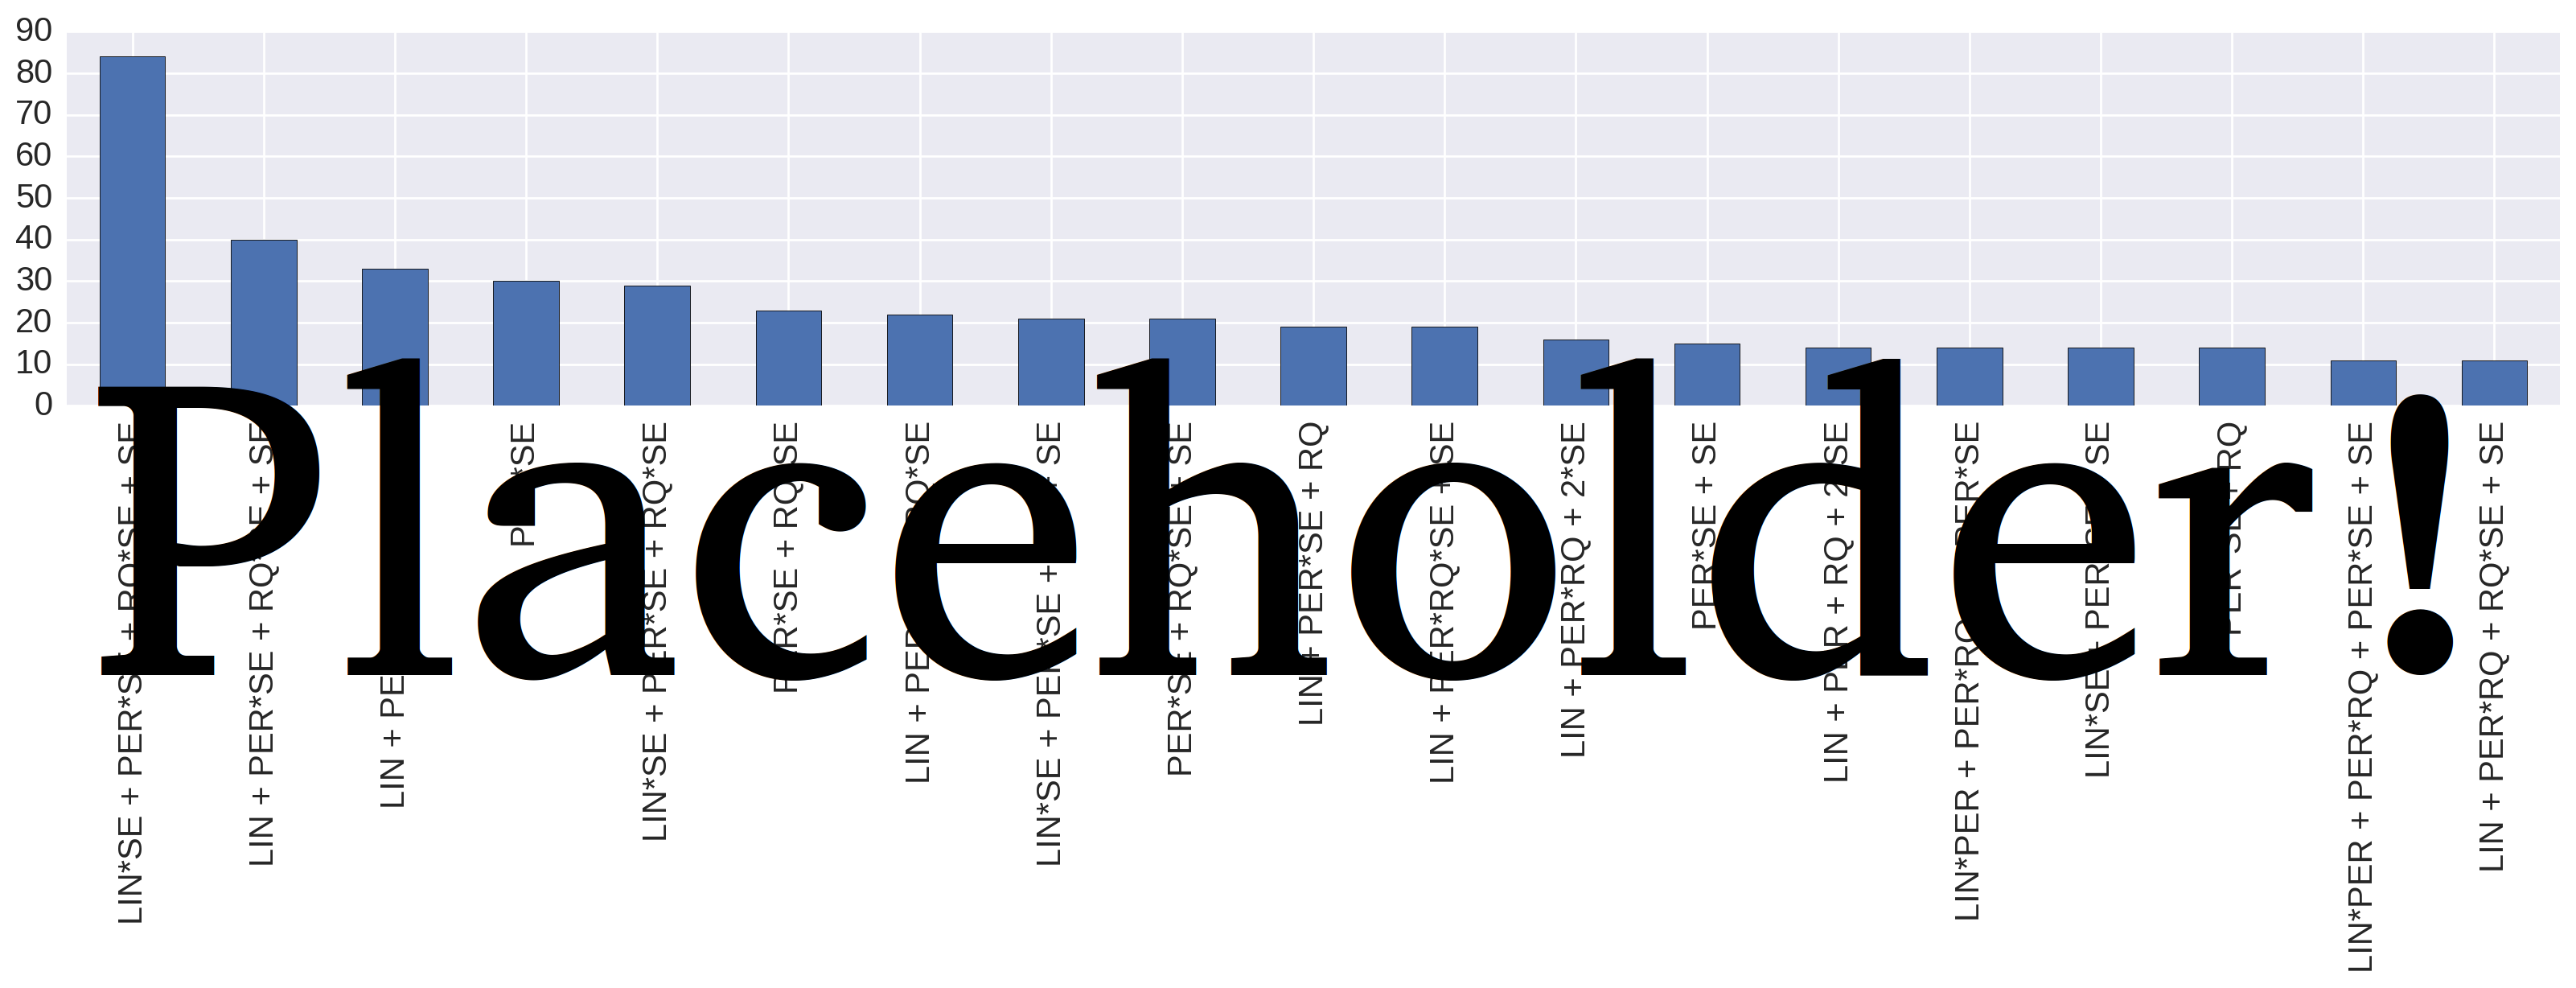
\includegraphics[width=0.7\linewidth]{structureCo2b.png}
%\captionof{figure}{\color{DarkSlateGray} Composition of covariance function parsed using the example SE $\times$ LIN $+$ PER $\times$ LIN $+$  RQ $\times$ LIN}
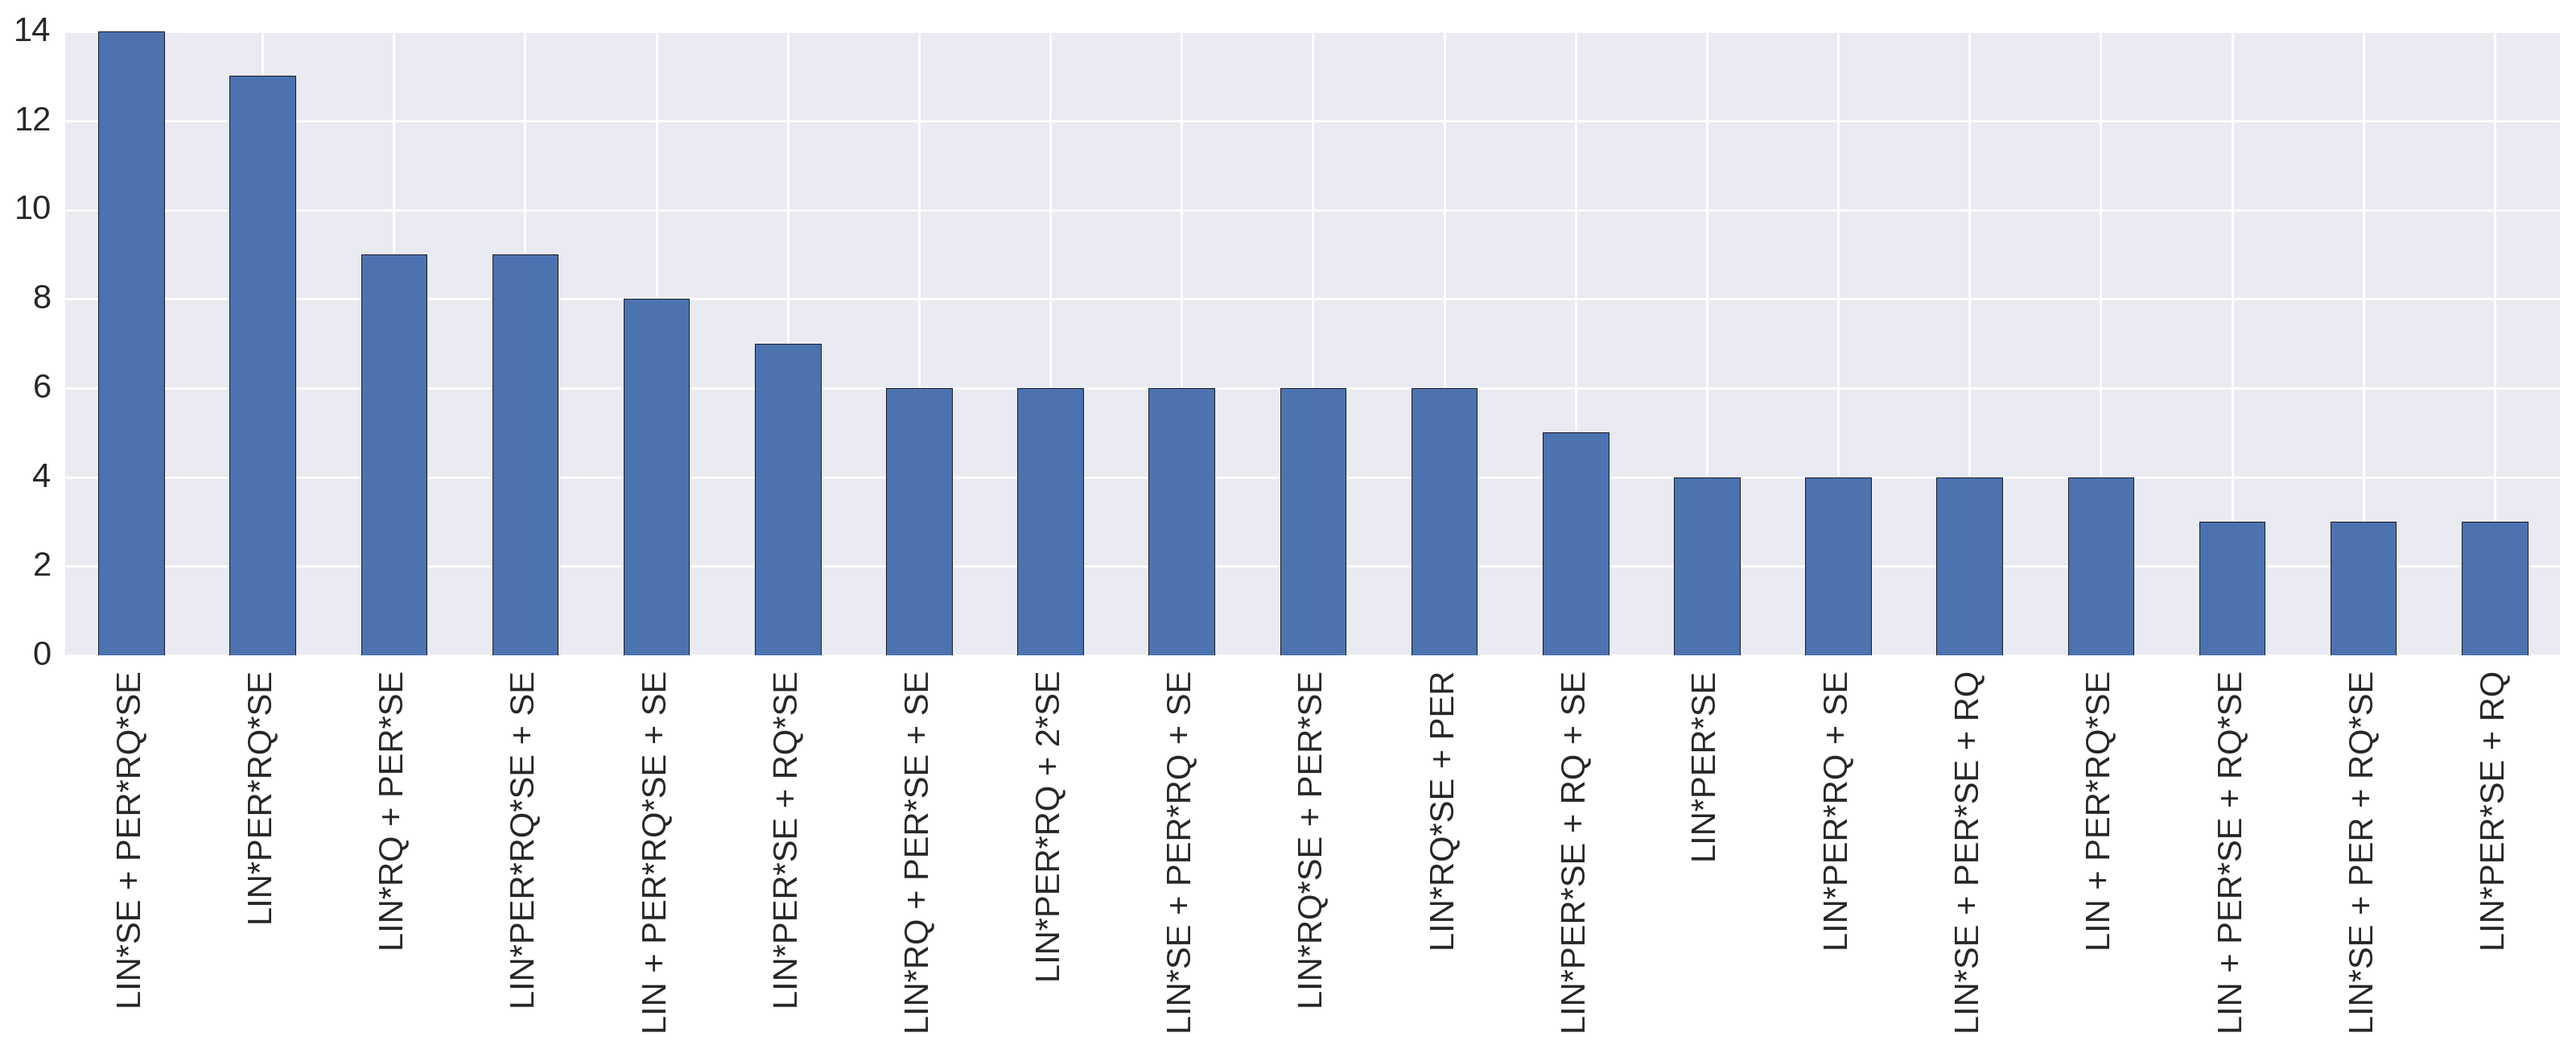
\includegraphics[width=0.7\linewidth]{structureAirlinec.png}
\end{center}\vspace{1cm}
 \begin{minipage}{\linewidth}
\small
\begin{lstlisting}[frame=single,label=alg:structureVent,caption=Venture Code for Bayesian GP Structure Learning,mathescape]
[ASSUME base_kernels (list K$_1$,K$_2$,$\cdots$,K$_n$)] % defined as above
[ASSUME p$_n$ (uniform_structure n)]        % prior on the number of kernels
[ASSUME S$_{\emph{K}}$ (subset  base_kernels p$_n$)]    % sampling a subset of size n
[ASSUME composition (lambda (l)          % kernel composition
                     (if (lte ( size l) 1)
                         (first l)
                          (if (flip)
                              (func_plus (first l) (cov_compo (rest l)))
                              (func_times (first l) (cov_compo (rest l)))
                          )
                     )
              )

[ASSUME K (composition  S$_{\emph{K}}$)]

[ASSUME (list f_compute f_emu) (gpmem f_restr K )]

for i=1 to n:
  [PREDICT (f_compute x[i])] % observing with a look-up function

[INFER  (REPEAT 2000 (DO 
                        (MH p$_n$ one 1) 
                        (MH S$_{\emph{K}}$ one 1) 
                        (MH K$^*$ one 1) 
                        (MH {hyper-parameters} one 10)) ]


\end{lstlisting}

\end{minipage}
 \subsection*{Decomposing a candidate Structure}
\begin{center}\vspace{1cm}
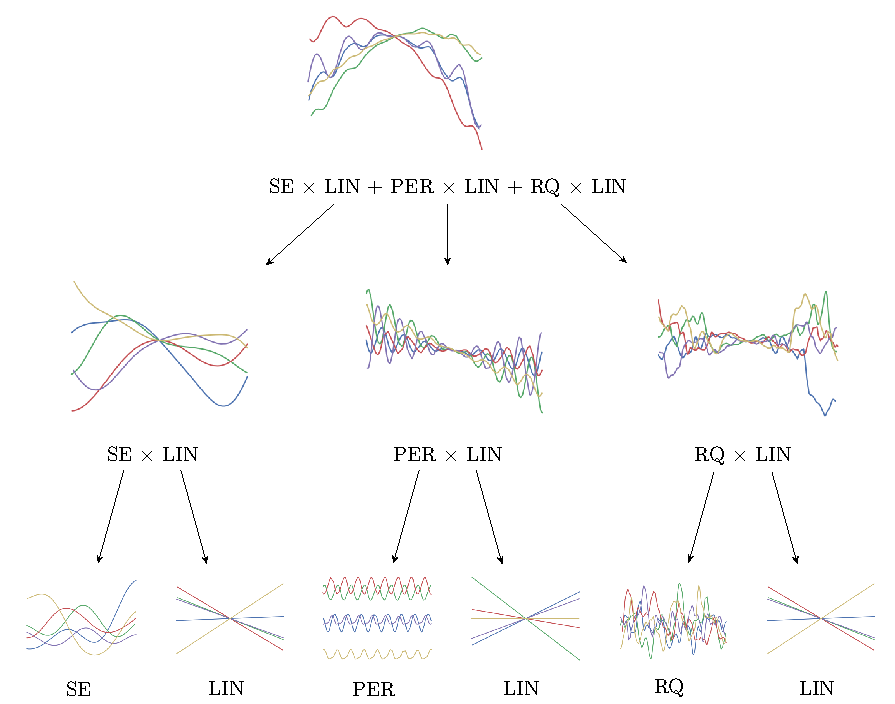
\includegraphics[width=0.7\linewidth]{parseTree.pdf}
%\captionof{figure}{\color{DarkSlateGray} Composition of covariance function parsed using the example SE $\times$ LIN $+$ PER $\times$ LIN $+$  RQ $\times$ LIN}
\end{center}\vspace{1cm}
 



---------------------------------------------------------------------

%----------------------------------------------------------------------------------------
%	Bayesian Optimization
%----------------------------------------------------------------------------------------
\section*{Bayesian Optimization}
\begin{wraptable}{r}{20cm} % Left or right alignment is specified in the first bracket, the width of the table is in the second
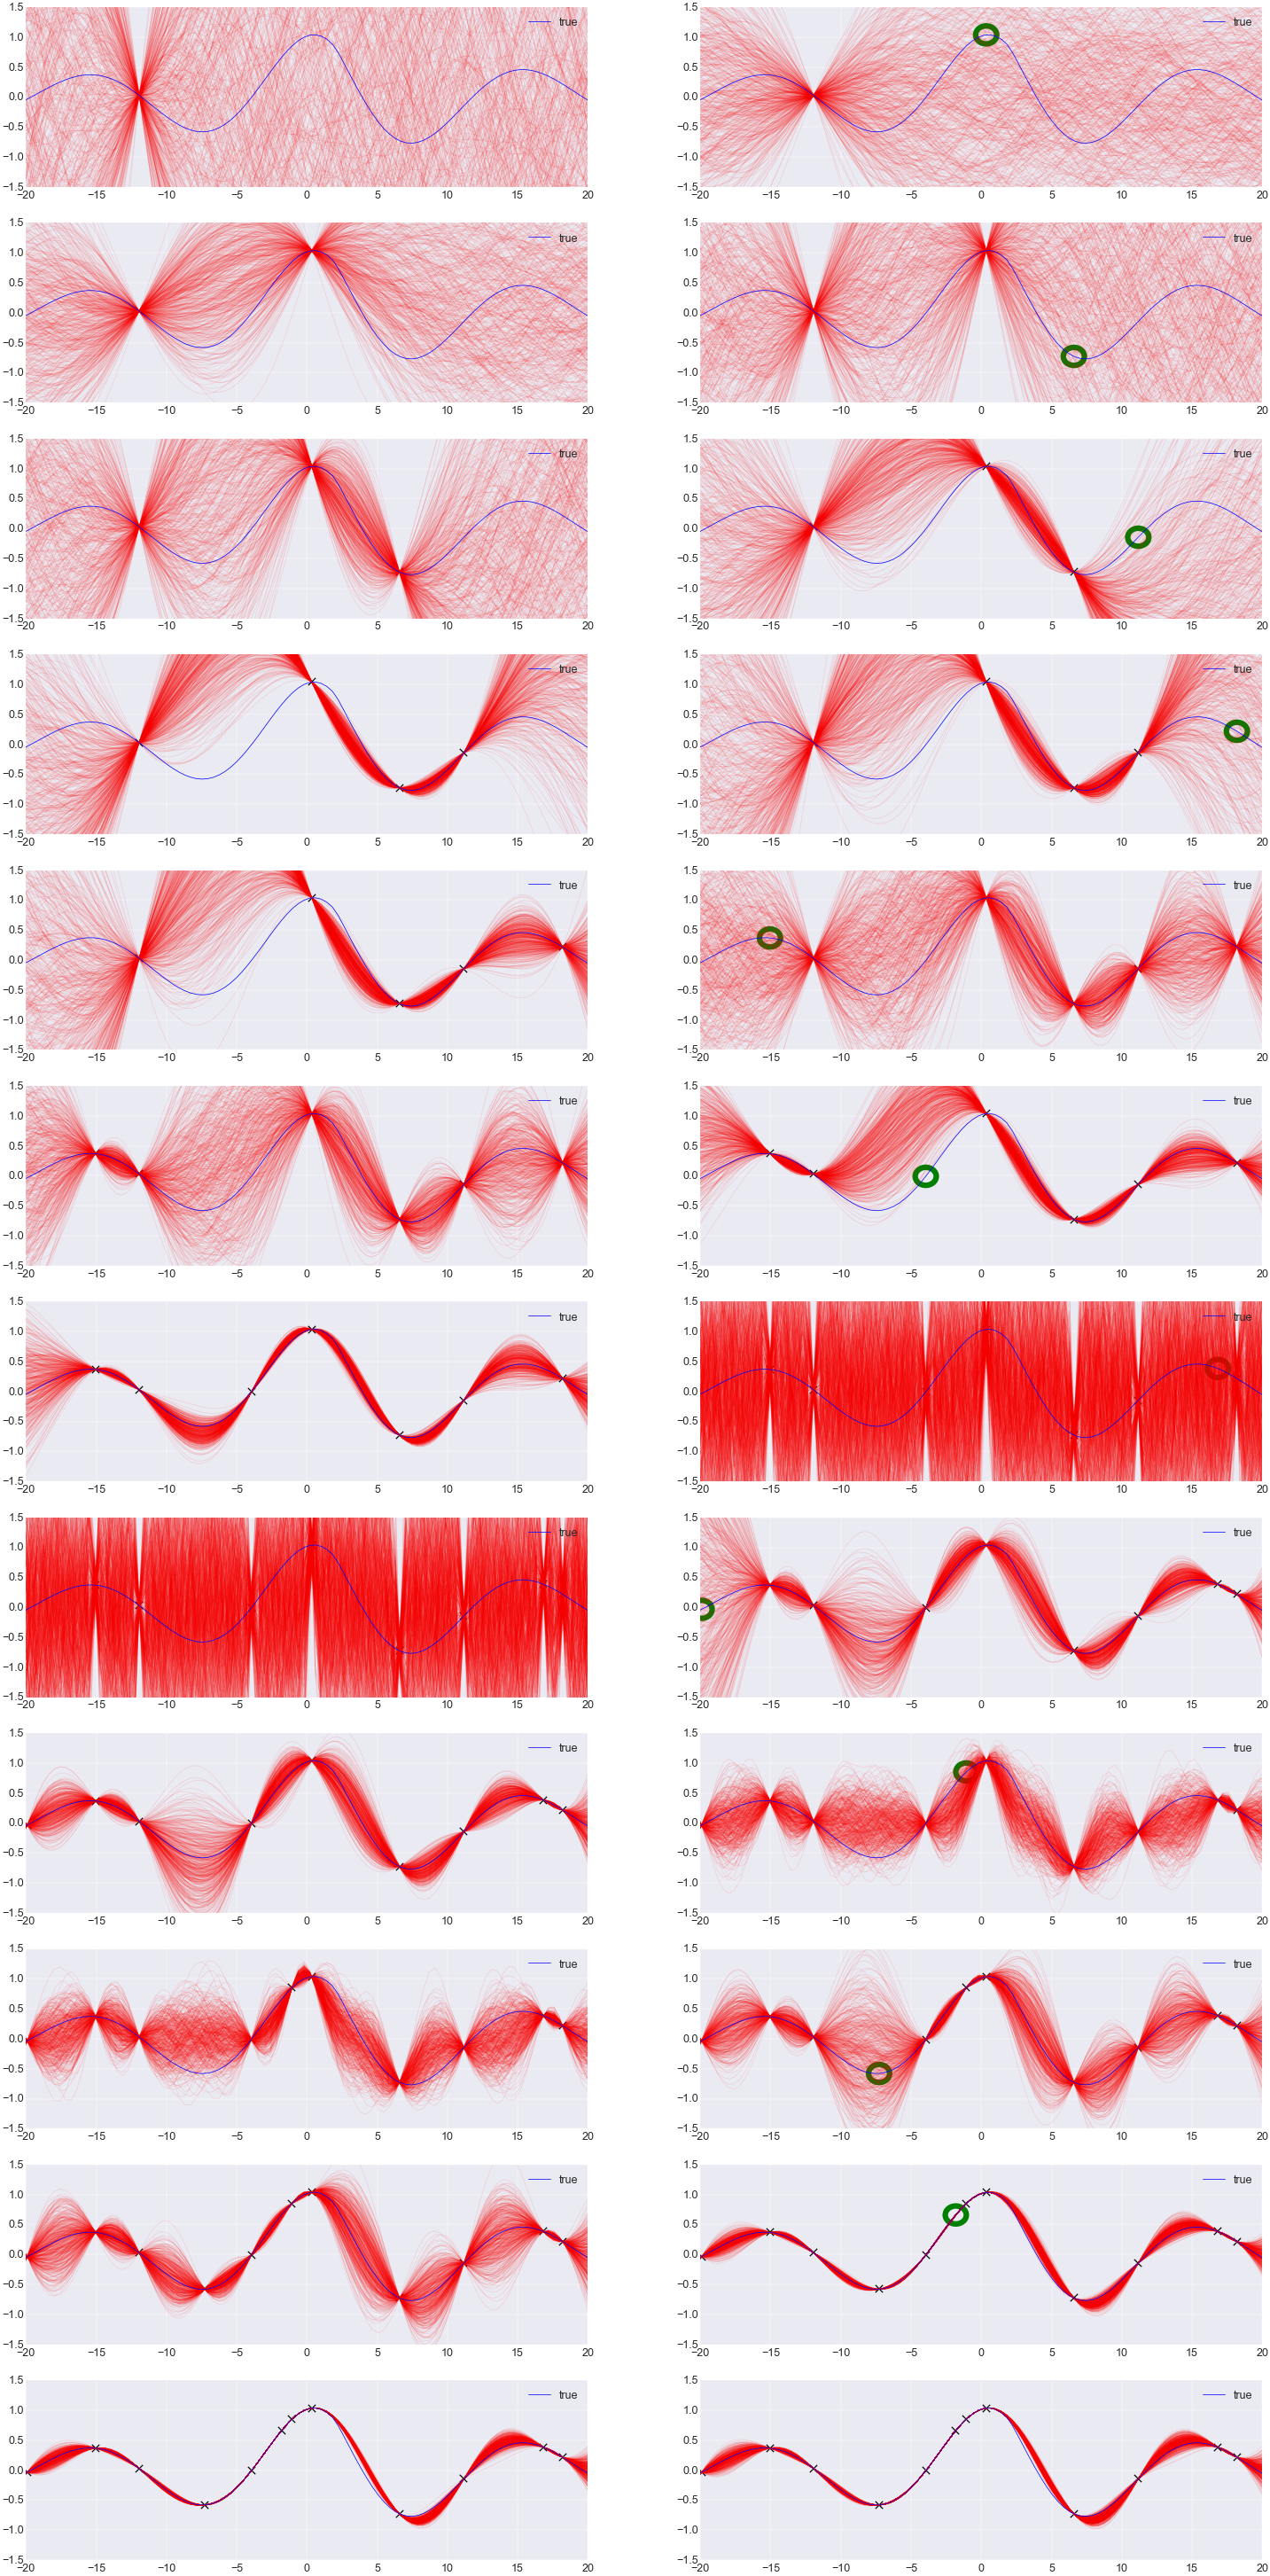
\includegraphics[width=20cm]{BayesOpt_gpmem_sequence.png}
\end{wraptable}
%Bayesian Optimization with Thompson sampling providing:
%\begin{itemize}
% \item  the ability to search over a broader space of contexts than the parametric families that are typically used;
% \item parsimony of the resulting probabilistic program.
%\end{itemize}
\subsection*{Thompson Sampling}
In Thompson sampling, the goal is to maximize the total reward received for all actions by placing a prior distribution $P(\theta)$ on the possible ``contexts'' $\theta \in \Theta$ with reward  $r \in \R$.

Repeat:
\begin{enumerate}
 \item Sample a context $\theta \sim P(\theta)$.
 \item Choose an action $a \in \Acal$ which (approximately) maximizes $V(a|\theta) = \Ebkt{r|a,\theta}$.
 \item\label{itm:Thompson-conditioning}
    Let $r_\true$ be the reward received for action $a$.
    Update the believed distribution on $\theta$, i.e., $P(\theta) \gets P_\rmnew(\theta)$ where $P_\rmnew(\theta) = P\pn{\theta \mvert a \mapsto r_\true}$.
\end{enumerate}

\subsection*{Bayesian Optimization with {\tt gpmem}}
\begin{itemize}
\item contexts $\theta = (\mu, K)$ are Gaussian processes over the action space $\Acal = \R$.
  \item $K_\prior = K_{\prior,\sigma,\ell}$ is a procedure, with parameters $\sigma,\ell$, to be used as the prior covariance function: $K_\prior(a,a') = \sigma^2 \exp\pn{-\frac{(a-a')^2}{2\ell^2}}$
  \item $\sigma$ and $\ell$ are (hyper)parameters for $K_\prior$
  \item $\abf_\past = \pn{a_i}_{i=1}^{n}$ are the previously probed actions
  \item $\rbf_\past = \pn{r_i}_{i=1}^{n}$ are the corresponding rewards
\end{itemize}

\subsection*{Above: Dynamics of Thompson sampling}
\begin{itemize}
 \item the blue curve is the true function $V$;
 \item the red region is a blending of 100 samples of the curve generated (jointly) by a GP-based emulator $V_\emu$;
 \item  the left and right columns show the state of $V_\emu$ before and after hyperparameter inference
 \item in the right column, the next chosen probe point is circled in green;
 \item each successive probe point $a$ is the (stochastic) maximum of $V_\emu$, sampled pointwise and conditioned on the values of the previously probed points; and
 \item probes tend to happen at points either where the value of $V_\emu$ is high, or where $V_\emu$ has high uncertainty.
 
\end{itemize}

      
     
     
      
    
%
%\begin{center}\vspace{1cm}
%\captionof{figure}{\color{DarkSlateGray} } \label{fig:bayesopt-sequence}
%\end{center}

   



\section*{Conclusions}
{\tt gpmem} is a generalization of a number of GP related models and can be applied to:
\begin{itemize}
\setlength{\itemindent}{1cm}
\item Hierarchical Bayesian GP
\item Kernel Structure Learning
\item Bayesian Optimization
\end{itemize}

\color{DarkSlateGray} % Set the color back to DarkSlateGray for the rest of the content

%----------------------------------------------------------------------------------------
%	FORTHCOMING RESEARCH
%----------------------------------------------------------------------------------------

%\section*{Forthcoming Research}

%Vivamus molestie, risus tempor vehicula mattis, libero arcu volutpat purus, sed blandit sem nibh eget turpis. Maecenas rutrum dui %blandit lorem vulputate gravida. Praesent venenatis mi vel lorem tempor at varius diam sagittis. Nam eu leo id turpis interdum %luctus a sed augue. Nam tellus.

 %----------------------------------------------------------------------------------------
%	REFERENCES
%----------------------------------------------------------------------------------------


\bibliographystyle{plain} % Plain referencing style
\bibliography{June2015} % Use the example bibliography file sample.bib

%----------------------------------------------------------------------------------------
%	ACKNOWLEDGEMENTS
%----------------------------------------------------------------------------------------

%\section*{Acknowledgements}


%----------------------------------------------------------------------------------------

\end{multicols}
\end{document}